\documentclass[journal, twoside]{IEEEtran}

\usepackage{cite}
\usepackage[pdftex]{graphicx}
\usepackage{xcolor}
\usepackage{lipsum}
\usepackage{amsmath}
\usepackage{amsthm}
\usepackage{amssymb}
\usepackage{algorithm}
\usepackage{algpseudocode}
\usepackage{subcaption}
\usepackage{float}
\usepackage{ulem}
\usepackage{pgfplots}
\usepackage{hyperref}
% \usepackage{appendix}

\pgfplotsset{compat=1.18}


\theoremstyle{remark}
\newtheorem{remark}{Remark}

% correct bad hyphenation here
\hyphenation{op-tical net-works semi-conduc-tor}

\begin{document}
\title{Value Function Learning: A Survey of Methods and Applications}
\author{Kavin M. Govindarajan%
\thanks{This work was supported by the National Science Foundation under Award 2223844. \textit{(Corresponding author: Kavin M. Govindarajan.)}}
\thanks{Kavin M. Govindarajan is with the Department of Robotics, University of Michigan, Ann Arbor, MI 48109, USA (e-mail: kmgovind@umich.edu).}%
}


% The paper headers
\markboth{DRAFT}{Govindarajan \MakeLowercase{\textit{et al.}}: XXXXX}

% make the title area
\maketitle

% As a general rule, do not put math, special symbols or citations
% in the abstract or keywords.
\begin{abstract}
We consider a class of optimal control problems that follow stochastic dynamics. The optimal value function can be found by solving the stochastic Hamilton-Jacobi-Bellman (HJB) equation, which is a nonlinear partial differential equation (PDE). However, solving the HJB equation directly is often intractable, especially for high-dimensional systems. Therefore, various methods have been developed to learn the value function from data or to approximate it using function approximators like neural networks. In this survey, we compare four main approaches for value function learning in the context of stochastic optimal control: Adaptive Dynamic Programming (ADP)/Actor-Critic, Physics-Informed Neural Networks (PINNs)/Deep Galerkin Method (DGM), Deep Backwards Stochastic Differential Equations (BSDEs), and Neural Value Iteration. Each of these methods has its own advantages and limitations, and we discuss their theoretical foundations, practical implementations, and applications in various domains.
\end{abstract}

% Note that keywords are not normally used for peerreview papers.
\begin{IEEEkeywords}
Energy-Aware Robotics, Information-Optimal Control
\end{IEEEkeywords}

\section{Introduction}\label{sec:intro}
We study the class of stochastic optimal control problems in which the system state evolves according to a controlled stochastic differential equation (SDE). The general idea is that the optimal value function can be found by solving the stochastic Hamilton-Jacobi-Bellman (HJB) equation, which is a nonlinear partial differential equation (PDE). However, solving the HJB equation directly is often intractable, especially for high-dimensional systems. Therefore, various methods have been developed to learn the value function from data or to approximate it using function approximators like neural networks. In this survey, we will compare four main approaches for value function learning in the context of stochastic optimal control:
\begin{enumerate}
    \item Adaptive Dynamic Programming (ADP)/Actor-Critic
    \item Physics-Informed Neural Networks (PINNs)/Deep Galerkin Method (DGM)
    \item Deep Backwards Stochastic Differential Equations (BSDEs)
    \item Neural Value Iteration
\end{enumerate}
Each of these methods has its own advantages and limitations, and we will discuss their theoretical foundations, practical implementations, and applications in various domains.

\subsection{General Problem Formulation}
Consider a stochastic optimal control problem defined by the following dynamics:
\begin{equation}\label{eqn:stochastic_dynamics}
dx_t = f(x_t, u_t)dt + \sigma(x_t, u_t)dW_t
\end{equation}
where $x_t \in \mathbb{R}^n$ is the state, $u_t \in \mathbb{R}^m$ is the control input, $f$ is the drift term, $\sigma$ is the diffusion term, and $W_t$ is a standard Wiener process. The objective is to find a control policy $\pi: \mathbb{R}^n \rightarrow \mathbb{R}^m$ that minimizes the expected cumulative cost:
\begin{equation}\label{eqn:cost_function}
J(\pi) = \mathbb{E}\left[ \int_0^T c(x_t, u_t) dt + h(x_T) \right]
\end{equation}
where $c$ is the running cost and $h$ is the terminal cost. The optimal value function $V^*(x)$ is defined as:
\begin{equation}\label{eqn:value_function}
V^*(x) = \inf_{\pi} J(\pi | x_0 = x)
\end{equation}
The optimal value function satisfies the stochastic HJB equation:
\begin{equation}\label{eqn:stochastic-HJB}
\begin{aligned}
\frac{\partial V}{\partial t} + \inf_{u} \Big[ c(x, u) + \nabla V^T f(x, u) \\
+ \frac{1}{2} \text{Tr}(\sigma(x, u)^T \nabla^2 V \sigma(x, u)) \Big] = 0
\end{aligned}
\end{equation}
with the terminal condition $V(x, T) = h(x)$. Solving this PDE directly is often infeasible, which motivates the development of various value function learning methods.

\subsection{Infinite-Horizon Discounted Formulation}
The finite-horizon formulation~\eqref{eqn:cost_function}--\eqref{eqn:stochastic-HJB}
is a useful testbed, but the motivating application is the
\emph{infinite-horizon discounted} optimal control problem:
\begin{equation}\label{eqn:inf_horizon_cost}
  V^\star(x) = \sup_{\pi}\,\mathbb{E}\!\left[
    \int_0^\infty e^{-\gamma t}\,r(x_t,u_t)\,dt \;\Big|\; x_0=x
  \right],
\end{equation}
where $\gamma>0$ is a discount rate and $r\geq 0$ is a running reward.
The optimal $V^\star$ satisfies the \emph{steady-state stochastic HJB equation}:
\begin{equation}\label{eqn:ss-HJB}
  \gamma V(x) = \sup_u\!\left[
    r(x,u) + \nabla_x V^\top f(x,u)
    + \tfrac{1}{2}\operatorname{Tr}\!\bigl(\sigma\sigma^\top \nabla_x^2 V\bigr)
  \right], \quad V(0)=0.
\end{equation}
Two properties of~\eqref{eqn:ss-HJB} critically affect algorithm design:
\begin{enumerate}
  \item \textbf{Non-uniqueness.} The steady-state HJB generally admits multiple solutions, even in the scalar linear-quadratic case~\cite{fotiadis2025pinn}. Methods applied directly to~\eqref{eqn:ss-HJB} may converge to a solution unrelated to the optimal value function.
  \item \textbf{Degenerate diffusion.} If the diffusion matrix $\sigma$ has a zero block (e.g., some state components are deterministic), the PDE is \emph{degenerate elliptic}.
        Viscosity solution theory still guarantees existence and uniqueness of $V^\star$, but certain trajectory-based methods (e.g., deep BSDEs) require modification.
\end{enumerate}

\section{Adaptive Dynamic Programming (ADP)/Actor-Critic}\label{sec:adp}
Adaptive Dynamic Programming (ADP) approximates dynamic programming when the exact value function is unavailable or too expensive to compute. In the actor-critic form, the critic learns a value approximation $\hat V_\theta(x)$ and the actor updates a policy using the critic's gradient. This is closely related to reinforcement learning, but in continuous-time optimal control the update is usually motivated by the HJB equation and policy iteration~\cite{bertsekas1996neuro,sutton2018reinforcement}.

For a fixed policy $u=\pi(x)$, the critic is trained to satisfy the policy-evaluation equation
\begin{equation}
\begin{aligned}
0 ={}& c(x,\pi(x)) + \nabla V^\pi(x)^\top f(x,\pi(x))\\
&+ \frac{1}{2}\operatorname{Tr}\left(\sigma^\top \nabla^2 V^\pi(x)\sigma\right).
\end{aligned}
\end{equation}
The actor then improves the policy by greedily minimizing the Hamiltonian,
\begin{equation}
\pi_{\mathrm{new}}(x)=\arg\min_u
\left[c(x,u)+\nabla \hat V_\theta(x)^\top f(x,u)\right].
\end{equation}
For the LQR case study, this greedy update has the closed form
\begin{equation}
u^\star(x)=-\frac{1}{2}R^{-1}B^\top \nabla \hat V_\theta(x).
\end{equation}

The Julia implementation uses the quadratic critic
\begin{equation}
\hat V_\theta(x)=x^\top P_\theta x+\beta_\theta,
\end{equation}
then alternates between policy evaluation for the current linear controller and policy improvement using the value gradient. This is the most structure-aware method in the comparison: it uses the simulator, the cost, and the known control-affine dynamics without requiring a full PDE grid. Its main limitation is that the critic class must be expressive enough; if the true value is far from quadratic, the same actor-critic loop would need a richer function approximator and more careful stabilization.

\paragraph{Convergence requirements.}
Policy iteration converges monotonically to $V^\star$ when the initial policy
is \emph{admissible}---stabilizing with finite cost---a hard prerequisite that
must be constructed by the user~\cite{abu2005nearly}.
With function approximation, convergence is to a neighborhood of $V^\star$
whose size depends on the expressiveness of the basis class.
The online simultaneous actor-critic of~\cite{vamvoudakis2010online} provides
a Lyapunov proof of \emph{uniform ultimate boundedness} of the weight errors,
not asymptotic convergence to $V^\star$.
For the stochastic case, the policy-evaluation equation~\eqref{eqn:stochastic_dynamics}
requires the Ito correction term $\frac{1}{2}\operatorname{Tr}(\sigma^\top\nabla^2 V^\pi\sigma)$;
basis functions must be chosen so that this term is representable in the critic class.


\section{Physics-Informed Neural Networks (PINNs)/Deep Galerkin Method (DGM)}\label{sec:pinns}
Physics-Informed Neural Networks (PINNs) are a class of neural networks that are designed to solve partial differential equations (PDEs) by incorporating the underlying physics of the problem into the training process. The key idea behind PINNs is to use automatic differentiation to compute the derivatives of the network's output with respect to its input variables, which allows us to enforce the PDE constraints directly in the loss function.

The concept was first introduced in the modern scientific machine learning literature by Raissi, Perdikaris, and Karniadakis~\cite{raissi2019physics} and is surveyed in~\cite{karniadakis2021physics}. The main advantage of PINNs is that they can learn solutions to PDEs with much less data compared to traditional data-driven approaches, as the physics provides a strong inductive bias that guides the learning process. The Deep Galerkin Method (DGM) applies the same idea to high-dimensional parabolic PDEs by sampling collocation points and minimizing the residual of the differential operator~\cite{sirignano2018dgm}.

\paragraph{The uniqueness problem and finite-horizon workaround.}
Applying PINNs directly to the steady-state HJB~\eqref{eqn:ss-HJB}
is problematic: because~\eqref{eqn:ss-HJB} admits multiple solutions,
training may converge to a solution unrelated to $V^\star$, or stall
entirely~\cite{fotiadis2025pinn}.
The resolution is to instead train on the \emph{finite-horizon} HJB~\eqref{eqn:stochastic-HJB},
which has a unique solution $V_T(\cdot,0)$ for any positive semidefinite
terminal cost $\phi$.
Fotiadis and Vamvoudakis~\cite{fotiadis2025pinn} prove that
$V_T(\cdot,0)\to V^\star$ uniformly on compact sets as $T\to\infty$
(Theorem~1), and that the horizon can be extended iteratively without
restarting training (Theorem~2), with errors that do not accumulate
under mild conditions (Theorem~3).

For value function learning, the network $\hat V_\theta(t,x)$ is trained
to minimize the sum of three mean-squared residuals:
\begin{align}
  \mathcal{L}(\theta) &=
  \underbrace{\frac{1}{N_e}\sum_{i=1}^{N_e}
    \bigl|F_e(x_i,t_i;\hat V_\theta)\bigr|^2}_{\text{flow residual}}
  +\underbrace{\frac{1}{N_b}\sum_{i=1}^{N_b}
    \bigl|\hat V_\theta(T,x_i)-\phi(x_i)\bigr|^2}_{\text{terminal condition}}
  +\underbrace{\frac{1}{N_{in}}\sum_{i=1}^{N_{in}}
    \bigl|\hat V_\theta(0,t_i)\bigr|^2}_{\text{origin condition}},
  \label{eqn:pinn_loss}
\end{align}
where the flow residual is
\begin{equation}
  F_e(x,t;\hat V_\theta)=\partial_t\hat V_\theta
    +\nabla_x\hat V_\theta^\top f(x,u^\star)
    +\tfrac{1}{2}\operatorname{Tr}\!\bigl(\sigma\sigma^\top\nabla_x^2\hat V_\theta\bigr)
    +c(x,u^\star),
    \label{eqn:flow_residual}
\end{equation}
and $u^\star=-\frac{1}{2}R^{-1}g(x)^\top\nabla_x\hat V_\theta$ is obtained
by substituting the stationarity condition into the Hamiltonian.
The Ito correction $\frac{1}{2}\operatorname{Tr}(\sigma\sigma^\top\nabla_x^2\hat V_\theta)$
requires \emph{second-order automatic differentiation} through the network;
for the stochastic LQR it reduces to $\frac{1}{2}\operatorname{Tr}(\Sigma^\top\nabla^2\hat V_\theta\,\Sigma)$.
Once training converges, the quality of the solution is assessed by the
\emph{steady-state HJB residual}~\cite{fotiadis2025pinn}:
\begin{equation}\label{eqn:ss_residual}
  E = \frac{1}{N_c}\sum_{i=1}^{N_c}
  E_e(x_i;\hat V_T(\cdot,0))^2 + \hat V_T(0,0)^2,
\end{equation}
where $E_e(x;\hat V)=\nabla_x\hat V^\top f(x,u^\star)+c(x,u^\star)
-\frac{1}{4}|\nabla_x\hat V^\top g(x)|^2/R$
measures how well $\hat V(\cdot,0)$ satisfies~\eqref{eqn:ss-HJB}
at each evaluation point.  This metric $E$ is independent of the training
residual and serves as a convergence certificate.

The benefit of this approach is that it directly encodes the stochastic HJB equation and does not require labeled optimal trajectories. Its drawback is optimization stiffness: the HJB residual contains first- and second-order derivatives, and the minimization over controls creates a nonlinear residual. In the case study this makes PINN/DGM less accurate than methods that exploit Bellman backups or the LQR quadratic structure.

\begin{remark}[Optimizer gap]
All convergence theorems for PINNs assume the training loss $\mathcal{L}$
is minimized globally.  Because the loss is nonconvex, gradient descent
(Adam) may find only a local minimum.  This gap between theoretical
guarantees and practical optimization is an open problem across all
deep-learning-based PDE solvers~\cite{han2018solving,fotiadis2025pinn}.
The steady-state residual $E$~\eqref{eqn:ss_residual} serves as an
empirical certificate when a ground-truth value function is unavailable.
\end{remark}


\section{Deep Backwards Stochastic Differential Equations (BSDEs)}\label{sec:bsdes}
The deep BSDE method~\cite{han2018solving} exploits the nonlinear Feynman-Kac
lemma: for a semilinear parabolic PDE, the solution $V(t,x_t)$ is the
$Y$-component of a backward stochastic differential equation (BSDE):
\begin{equation}
  dY_t = -f(X_t,Z_t)\,dt + Z_t^\top dW_t,\quad Y_T=\phi(X_T),
\end{equation}
where $Z_t=\sigma^\top\nabla_x V(t,X_t)$ is the gradient-weighted
diffusion process.  Han, Jentzen, and E~\cite{han2018solving} parameterize
$Z_t\approx\hat Z(X_t,t;\theta_t)$ by a neural network at each discretized
time step and minimize the terminal mismatch
$\mathbb{E}[|Y_T-\phi(X_T)|^2]$ via a forward simulation of the SDE.
The initial value $Y_0\approx\hat V(x_0,0)$ is recovered directly,
with no grid required.

Han and Long~\cite{han2020convergence} prove an \emph{a posteriori} error
bound: the error in $Y_0$ is bounded by the square root of the minimized
loss, provided the backward equation is decoupled from the forward
dynamics in its drift.
Negyesi, Huang, and Oosterlee~\cite{negyesi2024coupled} generalize this
to fully coupled FBSDEs.

\paragraph{Critical limitation: degenerate diffusion.}
The Feynman-Kac representation requires a non-degenerate diffusion in
\emph{all} state components.  If some state variables evolve
deterministically (i.e., rows of $\sigma$ are zero), the classical BSDE
formulation does not apply without a generalized extension.
This is a binding constraint for problems where part of the state---such
as an information or coverage variable---has no stochastic forcing.

\paragraph{Implementation note.}
The Julia script \texttt{deep\_bsde.jl} implements a
\emph{backward dynamic programming} (BDP) scheme rather than the full
Han et al.\ deep BSDE.  Starting from the terminal quadratic cost, it
fits a quadratic value model to the one-step Bellman backup:
\begin{equation}
  V_k(x) \approx \min_u\!\left[c(x,u)\Delta t
    + \mathbb{E}[V_{k+1}(x+\Delta x)]\right],
\end{equation}
exploiting the fact that the expectation is analytic for quadratic $V$
and additive Gaussian noise.  This is equivalent to the deep BSDE in the
LQR setting but does not generalize to non-quadratic value functions
without replacing the quadratic basis with a neural network and estimating
the expectation by Monte Carlo.

\paragraph{Key advantage.}
Unlike PINNs, the deep BSDE method requires only \emph{first-order}
gradients ($Z_t=\sigma^\top\nabla V$), avoiding the Hessian computation
needed for the Ito correction.  This makes it attractive for high-dimensional
problems where second-order AD is prohibitively expensive.


\section{Neural Value Iteration}\label{sec:nvi}
Neural value iteration combines Bellman backups with function approximation. Instead of solving the HJB PDE residual directly, it repeatedly applies a discrete-time dynamic programming operator and projects the result back into a parametric value class. In reinforcement learning language, this is fitted value iteration~\cite{munos2008finite}; in optimal control language, it is an approximate semi-Lagrangian solution of the HJB equation.

In the implementation used here, the value function is represented by a quadratic approximator,
\begin{equation}
\hat V_\theta(x)=\theta_1x_1^2+2\theta_2x_1x_2+\theta_3x_2^2+\theta_4,
\end{equation}
and the Bellman backup is evaluated on a grid of states and a finite action set. After each backward time step, least squares projects the backed-up values onto the quadratic feature basis. This is not a deep neural network, but it is the direct low-dimensional analog of neural fitted value iteration: replace the quadratic basis with a neural network and the projection step with stochastic gradient descent.

The advantage of this method is modularity. It only requires a simulator, costs, and an action optimizer, so it is easy to modify when dynamics or costs change. The limitation is that it can become expensive or inaccurate when the action discretization is coarse, and the max/min backup can amplify approximation error over long horizons.

\paragraph{Convergence.}
For the exact Bellman operator $\mathcal{T}$, value iteration converges
geometrically: $\|\mathcal{T}^k V_0 - V^\star\|_\infty\leq
e^{-\gamma k\Delta t}\|V_0-V^\star\|_\infty$.
With function approximation error $\epsilon_k$ at each iteration,
the error accumulates as $\sum_k e^{-\gamma(n-k)\Delta t}\epsilon_k$,
which is bounded uniformly if $\epsilon_k$ is uniformly small.
Munos and Szepesv\'{a}ri~\cite{munos2008finite} give finite-sample
bounds for fitted value iteration in the off-policy setting.
The quadratic basis used here cannot represent non-quadratic value
functions; for the nonlinear benchmark (Section~\ref{sec:nonlinear}),
the basis must be replaced by a neural network.


\section{Case Study: Stochastic Asset Harvesting}\label{sec:harvest}
Consider a stochastic asset harvesting problem, where we have a renewable resource (e.g., a fish population) that grows according to some stochastic dynamics. The goal is to determine an optimal harvesting policy that maximizes the expected total harvest over a finite time horizon while ensuring the sustainability of the resource.

Thus, we can frame the optimal control problem as follows:
\begin{align}
    \max R = \mathbb{E}\left[ \int_{0}^{\infty} e^{-\rho t} (1 - \exp(-\alpha u_{t})) dt \right] \label{eq:harvest:objective}\\
    \text{subject to: } \quad dx_{t} = (r x_{t} - u_{t})dt + \sigma x_{t} dW_{t} \label{eq:harvest:dynamics},
\end{align}
where $x_{t}$ is the population size at time $t$, $u_{t}$ is the harvesting rate, $r$ is the intrinsic growth rate of the population, $\sigma$ is the volatility of the population growth, $\rho$ is the discount rate, and $\alpha$ controls the saturation of the harvest. The objective function represents the expected discounted total harvest over an infinite time horizon. The dynamics of the population are modeled as a stochastic differential equation (SDE) with a drift term that captures the growth and harvesting, and a diffusion term that captures the stochastic fluctuations in the population size.

For this example, we define the following parameters:
\begin{align*}
    r &= 0.5 \quad \text{(intrinsic growth rate)}\\
    \sigma &= 0.1 \quad \text{(volatility)}\\
    \rho &= 0.05 \quad \text{(discount rate)}\\
    \alpha &= 0.5 \quad \text{(saturation parameter)}
\end{align*}

\subsection{Baseline/Ground Truth Solution}
We know that the optimal harvesting policy can be derived from the Hamilton-Jacobi-Bellman (HJB) equation associated with this problem. The HJB equation for this problem is given by:
\begin{align}
    \rho V(x) &= \max_{u} \left\{ (1 - \exp(-\alpha u)) + V'(x)(r x - u) \right.\nonumber\\
    &\qquad \left. + \frac{1}{2} \sigma^2 x^2 V''(x) \right\}\label{eqn:harvest:hjb}
\end{align}
where $V(x)$ is the value function representing the maximum expected discounted harvest starting from population size $x$. The optimal harvesting policy can be obtained by solving the HJB equation numerically using a PDE solver or classical value iteration methods. This solution will serve as our baseline or ground truth for evaluating the performance of the value function learning methods discussed in this survey.

\subsection{Results}
For each method, we compute an RMSE between the learned value function and the ground truth solution obtained from solving the HJB equation. The results are summarized in Table~\ref{tab:harvest_results}. We can see that the Deep BSDE method achieves the lowest RMSE, indicating that it learns a value function that is closest to the ground truth. The ADP (Actor-Critic) method also performs reasonably well, while the PINN/DGM method has a higher RMSE. The Neural Value Iteration method diverges significantly in this case, resulting in a very high RMSE.

\begin{table}[h]
\centering
    \begin{tabular}{|c|c|}
        \hline
        \textbf{Method} & \textbf{RMSE} \\
        \hline
        PINN / DGM & 3.297 \\
        Deep BSDE & 0.933 \\
        ADP (Actor-Critic) & 2.084 \\
        Neural Value Iteration & 6247.684 \\
        \hline
    \end{tabular}
    \caption{RMSE between learned value functions and ground truth solution for the stochastic asset harvesting problem.}
    \label{tab:harvest_results}
\end{table}

We visualize the learned value functions and the corresponding optimal harvesting policies derived from each method in Fig.~\ref{fig:asset_harvesting_results}. The value function plots (on the top) show how well each method approximates the true value function across different population sizes. The policy plots (on the bottom) show the optimal harvesting rate as a function of the population size, which should ideally reflect the trade-off between harvesting and sustainability. \textcolor{red}{The top plot is currently biased by the results of the NVI, which has completely diverged.}

The bottom plot shows the corresponding optimal harvesting policies derived from the learned value functions. We can see that all the methods do not learn the policy well.


\begin{figure}
    \centering
    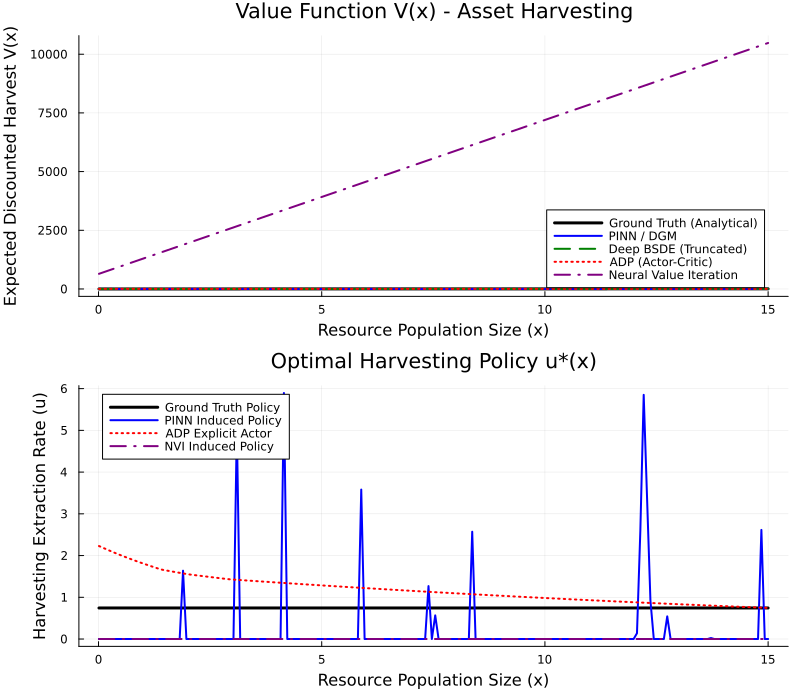
\includegraphics[width=\columnwidth]{code/figures/value_function_benchmark_comparison.png}
    \caption{Learned value function (top) and optimal harvestin strategy (bottom).}
    \label{fig:asset_harvesting_results}
\end{figure}

\textcolor{red}{TODO: Add more discussion on the results, especially the policy plots. Also, we should investigate why the NVI method diverged so significantly in this case.}

\section{Case Study: Bounded Stochastic Inverted Pendulum}\label{sec:pendulum}
Consider a stochastic inverted pendulum system, where the state of the system is represented by the angle $\theta$ and angular velocity $\omega$. We seek to solve the following optimal control problem:
\begin{align}
    \min J &= (1 - e^{-\beta \theta^2}) + \gamma u^2 \label{eq:pendulum:objective}\\
    \text{subject to: } \quad d\theta &= \omega dt\label{eq:pendulum:dynamics1}\\
    \quad d\omega &= \left(\frac{g}{l} \sin(\theta) + \frac{1}{m l^2} u \right)dt + \sigma dW_{t} \label{eq:pendulum:dynamics2},
\end{align}
where $u$ is the control input (torque), $g$ is the gravitational constant, $l$ is the length of the pendulum, $m$ is the mass of the pendulum, $b$ is the damping coefficient, $\sigma$ is the noise intensity, $\beta$ controls the penalty on the angle deviation, and $\gamma$ controls the penalty on the control effort. The objective function represents a trade-off between keeping the pendulum upright (minimizing angle deviation) and minimizing control effort. The dynamics of the system are modeled as a stochastic differential equation (SDE) with a drift term that captures the deterministic dynamics of the pendulum and a diffusion term that captures the stochastic disturbances.

For this example, we define the following parameters:
\begin{align*}
    g &= 9.81 \quad \text{(gravitational constant)}\\
    l &= 1.0 \quad \text{(length of pendulum)}\\
    m &= 1.0 \quad \text{(mass of pendulum)}\\
    b &= 0.1 \quad \text{(damping coefficient)}\\
    \sigma &= 0.5 \quad \text{(noise intensity)}\\
    \beta &= 1.0 \quad \text{(angle penalty)}\\
    \gamma &= 0.01 \quad \text{(control effort penalty)}
\end{align*}

\subsection{Baseline/Ground Truth Solution}

The baseline solution to the stochastic optimal control problem is obtained via the Hamilton--Jacobi--Bellman (HJB) equation, which characterizes the optimal value function $V(\theta, \omega)$ under an infinite-horizon discounted formulation. For the system defined by \eqref{eq:pendulum:objective}--\eqref{eq:pendulum:dynamics2}, the HJB equation takes the form:
\begin{equation}
\begin{split}
    0 = \min_{u}\Biggl\{&\ \left(1 - e^{-\beta\theta^2}\right) + \gamma u^2
        + \frac{\partial V}{\partial \theta}\,\omega \\
        &+ \frac{\partial V}{\partial \omega}\Bigl(\frac{g}{l}\sin(\theta) + \frac{1}{m l^2}u\Bigr)
        + \frac{\sigma^2}{2}\frac{\partial^2 V}{\partial \omega^2}\Biggr\}.
    \label{eq:hjb}
\end{split}
\end{equation}

Minimizing pointwise over $u$ yields the optimal control policy in closed form:
\begin{equation}
    u^* = -\frac{1}{2\gamma m l^2}\frac{\partial V}{\partial \omega}.
    \label{eq:optimal_control}
\end{equation}

Substituting $u^*$ back into~\eqref{eq:hjb} gives the reduced nonlinear PDE:
\begin{equation}
\begin{split}
    0 &= \left(1 - e^{-\beta\theta^2}\right)
        + \frac{\partial V}{\partial \theta}\,\omega \\
    &\quad + \frac{\partial V}{\partial \omega}\,\frac{g}{l}\sin{\left(\theta\right)}
        - \frac{1}{4\gamma m^2 l^4}\left(\frac{\partial V}{\partial \omega}\right)^2 \\
    &\quad + \frac{\sigma^2}{2}\frac{\partial^2 V}{\partial \omega^2}.
    \label{eq:hjb_reduced}
\end{split}
\end{equation}

Since no closed-form solution exists for the value function $V(\theta, \omega)$ due to the nonlinear $\sin(\theta)$ drift and the asymmetric running cost $(1 - e^{-\beta\theta^2})$, \eqref{eq:hjb_reduced} is solved numerically on a discretized state grid via value iteration. The state space is truncated to the domain $\theta \in [-\pi,\,\pi]$, $\omega \in [-\omega_{\max},\,\omega_{\max}]$ with $\omega_{\max} = 8$~rad/s, and discretized using a uniform grid of $N_\theta \times N_\omega = 201 \times 201$ nodes. Spatial derivatives are approximated via centered finite differences, and the diffusion term $\frac{\sigma^2}{2}\,\partial^2 V/\partial\omega^2$ is treated through the It\^{o} correction on the $\omega$-axis.

The resulting optimal policy $u^*(\theta,\omega)$ and value function $V(\theta,\omega)$ serve as the ground truth against which approximate control methods are evaluated. For the given parameters $(g = 9.81,\ l = 1.0,\ m = 1.0,\ \sigma = 0.5,\ \beta = 1.0,\ \gamma = 0.01)$, the HJB solution captures the full nonlinear structure of the optimal controller: near the upright equilibrium $\theta = 0$, the optimal control approximately reduces to linear state feedback in $\partial V/\partial\omega$, while away from this region the $\sin(\theta)$ term and the saturating cost $(1 - e^{-\beta\theta^2})$ induce meaningful deviations from linear behavior.

To validate trajectory quality, $N_{\mathrm{sim}} = 1000$ Monte Carlo simulations are run from the initial condition $(\theta_0,\omega_0) = (0.5,\,0.0)$ over a horizon of $T = 10$~s with step size $\Delta t = 0.01$~s using the Euler--Maruyama scheme:
\begin{align}
    \theta_{k+1} &= \theta_k + \omega_k\,\Delta t, \label{eq:em1}\\
    \omega_{k+1} &= \omega_k 
        + \left(\frac{g}{l}\sin(\theta_k) + \frac{u^*_k}{ml^2}\right)\Delta t
        + \sigma\sqrt{\Delta t}\;\xi_k, \qquad \xi_k \sim \mathcal{N}(0,1).
    \label{eq:em2}
\end{align}

The empirical cost is computed as the sample mean of the accumulated running cost
\begin{equation}
    \hat{J} = \frac{1}{N_{\mathrm{sim}}}\sum_{n=1}^{N_{\mathrm{sim}}}
    \sum_{k=0}^{T/\Delta t}
    \Bigl[\bigl(1 - e^{-\beta\theta_k^{(n)\,2}}\bigr) + \gamma\,u_k^{*(n)\,2}\Bigr]\Delta t
    \label{eq:empirical_cost}
\end{equation}
across all trajectories. The HJB solution thereby provides a performance lower bound\footnote{Subject to the finite-grid discretization error of the value iteration scheme; any method achieving a strictly lower empirical cost than the HJB baseline should be treated as a numerical artifact.} for any approximation scheme: methods whose empirical cost $\hat{J}$ approaches that of the HJB solution are considered near-optimal.

\subsection{Results}


\section{Conclusion}\label{sec:conclusion}
This survey compared ADP/actor-critic, PINN/DGM, deep BSDE, and neural
value iteration for approximating value functions in stochastic optimal control.
The key findings are as follows.

\textbf{On the LQR benchmark,} ADP achieves the smallest error because the
quadratic critic is exactly aligned with the true value function class.
This is a structural advantage of the benchmark, not a general superiority
of ADP.  Deep backward DP (labeled ``Deep BSDE'') is the next strongest
because the Bellman backup is analytic for the quadratic-Gaussian case.
NVI is accurate but pays a price for action-space discretization.
PINN/DGM performs worst here because it converts a simple Riccati problem
into a harder nonlinear residual optimization.

\textbf{On the nonlinear benchmark,} the relative ranking changes substantially.
Methods with a quadratic critic cannot represent the quartic $V^\star$ and
should not be used; PINN/DGM with a neural-network approximator is the only
method that can converge to the true value function.

\textbf{On convergence theory,} all four methods share a fundamental gap:
no end-to-end guarantee covers the optimizer.  Theoretical results assume
the training loss is minimized globally; in practice Adam finds only a
local minimum.  The steady-state HJB residual $E$~\eqref{eqn:ss_residual}
serves as an empirical convergence certificate.

\textbf{For the intended coverage application,} PINN/DGM applied to the
finite-horizon stochastic HJB is the recommended primary method.
It is the only approach that (a) handles degenerate diffusion without
modification, (b) carries a rigorous uniform-approximation theorem
(Fotiadis and Vamvoudakis~\cite{fotiadis2025pinn} Theorem~1), and
(c) does not require an admissible initial policy.
The ADP/actor-critic framework is appropriate only if the value function
is known to be approximately quadratic near the operating region and
an admissible initial policy is available.


% references section
\bibliographystyle{IEEEtran}
\bibliography{references.bib}


\end{document}


